\documentclass{article}
\usepackage{booktabs}
\usepackage{amsmath}
\usepackage{amssymb}
\usepackage[noend]{algorithmic}
\usepackage[nothing]{algorithm}
\usepackage{tikz}
\usepackage{latexsym}
\usepackage{float}
\usepackage{mathrsfs}
\providecommand{\e}[1]{\ensuremath{\times 10^{#1}}}
\renewcommand{\thealgorithm}{}
\usetikzlibrary{arrows}
\title{CS 522: Data Structures and Algorithms II \\ Homework 1}
\author{Dustin Ingram}
\begin{document}
\maketitle
\begin{enumerate}
    \item \textbf{Solution:}
    If both \textsc{Increment} and \textsc{Decrement} operations were included
    in the $k$-bit counter, an amortized analysis of the cost of $n$ operations
    would cost as much as $\Theta(nk)$ time because we would no longer be able
    to consider each operation as a consecutive \textsc{Increment}, but rather
    as any combination of \textsc{Increment}s and \textsc{Decrement}s. Thus, in
    a worse-case scenario, it would be possible to alternate $n$ times between
    two operations which cost $O(k)$ each, resulting in a total cost of
    $\Theta(nk)$.

    \item \textbf{Solution:}
    To show that the amortized cost of \textsc{Table-Delete} under this strategy
    is bounded above by a constant, we will consider two cases. We will use the
    potential function:

    $$ \Phi(T) = | 2\cdot T.num - T.size | $$

    The first case is the one in which the table does not contract, and thus
    $num_{i} = num_{i-1}-1$, $size_{i} = size_{i-1}$, and $c_{i} = 1$:

    \begin{eqnarray*}
        \hat{c_{i}} &=& c_{i} + \Phi_{i} - \Phi_{i-1} \\
        \hat{c_{i}} &=& 1 + |2\cdot num_{i} - size_{i}| - | 2\cdot num_{i-1} - size_{i-1} | \\
        \hat{c_{i}} &=& 1 + |2\cdot(num_{i-1} - 1) - size_{i-1}| - | 2\cdot num_{i-1} - size_{i-1} | \\
        \hat{c_{i}} &=& 1 + |-2| \\
        \hat{c_{i}} &=& 3 \\
    \end{eqnarray*}

    The second case is the one in which the table does contract, and thus
    $size_{i} = \frac{2}{3}size_{i-1}$, $num_{i-1} = \frac{1}{3}size_{i-1}$, and
    $c_{i} = num_{i} + 1$:

    \begin{eqnarray*}
        \hat{c_{i}} &=& c_{i} + \Phi_{i} - \Phi_{i-1} \\
        \hat{c_{i}} &=& (num_{i} +1) + |2\cdot num_{i} - size_{i}| - | 2\cdot num_{i-1} - size_{i-1} | \\
        \hat{c_{i}} &=& ((num_{i-1} - 1) + 1) + |2\cdot(num_{i-1} - 1) - \frac{2}{3}size_{i-1}| - | 2\cdot num_{i-1} - size_{i-1} | \\
        \hat{c_{i}} &=& (num_{i-1}) + |-2 + \frac{1}{3}size_{i-1}| \\
        \hat{c_{i}} &=& 2 \\
    \end{eqnarray*}

    Thus we see that the amortized cost of \textsc{Table-Delete} is at most 3
    and is thus bounded.

    \item \textbf{Solution:}
    One can use the following sequence to produce a Fibonacci heap that is only
    a linear chain of $n$ nodes. Since we start at the base case (where the heap
    is empty) and create a chain of a single node, followed by a chain of two
    nodes from a chain of one node, and then a chain of three nodes from a chain
    of two nodes, we can repeat the process $n$ times to produce a chain of
    total length $n$.

    \textsc{Fib-Heap-Insert}(H, $m$):
    \begin{figure}[H]
    \centering
    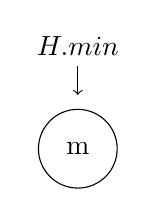
\begin{tikzpicture}[
      level 1/.style={sibling distance=48mm, level distance=10mm},
      level 2/.style={sibling distance=16mm, level distance=10mm},
      level 3/.style={sibling distance=8mm, level distance=10mm},
    ]
    \node [circle,draw, minimum size=1cm] (1){m};
    \node [above of=1, yshift=.3cm] (min) {$H.min$};
    \path [draw, ->, shorten >=5pt] (min)--(1.north);
    \end{tikzpicture}
    \end{figure}

    \textsc{Fib-Heap-Insert}(H, $m-1$):
    \begin{figure}[H]
    \centering
    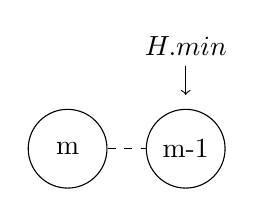
\begin{tikzpicture}[
      level 1/.style={sibling distance=100mm, level distance=10mm},
      level 2/.style={sibling distance=16mm, level distance=10mm},
      level 3/.style={sibling distance=100mm, level distance=10mm},
      node distance=1.5cm
    ]
    \node [circle,draw, minimum size=1cm] (1){m};
    \node [circle,draw, minimum size=1cm, right of=1] (2){m-1};
    \path [draw, dashed] (1)--(2);
    \node [above of=2, yshift=-.2cm] (min) {$H.min$};
    \path [draw, ->, shorten >=5pt] (min)--(2.north);
    \end{tikzpicture}
    \end{figure}

    \textsc{Fib-Heap-Insert}(H, $m-2$):
    \begin{figure}[H]
    \centering
    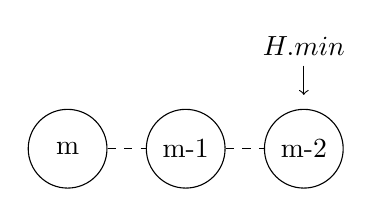
\begin{tikzpicture}[
      level 1/.style={sibling distance=48mm, level distance=10mm},
      level 2/.style={sibling distance=16mm, level distance=10mm},
      level 3/.style={sibling distance=8mm, level distance=10mm},
      node distance=1.5cm
    ]
    \node [circle,draw, minimum size=1cm] (1){m};
    \node [circle,draw, minimum size=1cm, right of=1] (2){m-1};
    \node [circle,draw, minimum size=1cm, right of=2] (3){m-2};
    \path [draw, dashed] (1)--(2);
    \path [draw, dashed] (2)--(3);
    \node [above of=3, yshift=-.2cm] (min) {$H.min$};
    \path [draw, ->, shorten >=5pt] (min)--(3.north);
    \end{tikzpicture}
    \end{figure}

    \textsc{Fib-Heap-Extract-Min}(H):
    \begin{figure}[H]
    \centering
    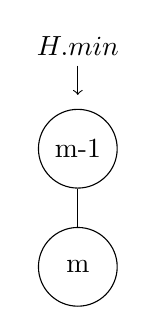
\begin{tikzpicture}[
      level 1/.style={sibling distance=48mm, level distance=10mm},
      level 2/.style={sibling distance=16mm, level distance=10mm},
      level 3/.style={sibling distance=8mm, level distance=10mm},
      node distance=1.5cm
    ]
    \node [circle,draw, minimum size=1cm] (1){m-1}
     child {node [circle,draw, minimum size=1cm, below of=1] (3){m}};
    \node [above of=1, yshift=-.2cm] (min) {$H.min$};
    \path [draw, ->, shorten >=5pt] (min)--(1.north);
    \end{tikzpicture}
    \end{figure}

    \textsc{Fib-Heap-Insert}(H, $m-3$):
    \begin{figure}[H]
    \centering
    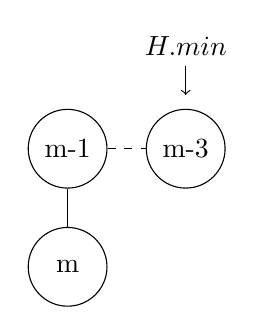
\begin{tikzpicture}[
      level 1/.style={sibling distance=48mm, level distance=10mm},
      level 2/.style={sibling distance=16mm, level distance=10mm},
      level 3/.style={sibling distance=8mm, level distance=10mm},
      node distance=1.5cm
    ]
    \node [circle,draw, minimum size=1cm] (1){m-1}
     child {node [circle,draw, minimum size=1cm, below of=1] (2){m}};
    \node [circle, draw, minimum size=1cm, right of=1] (4){m-3};
    \path [draw, dashed] (1)--(4);
    \node [above of=4, yshift=-.2cm] (min) {$H.min$};
    \path [draw, ->, shorten >=5pt] (min)--(4.north);
    \end{tikzpicture}
    \end{figure}

    \textsc{Fib-Heap-Insert}(H, $m-4$):
    \begin{figure}[H]
    \centering
    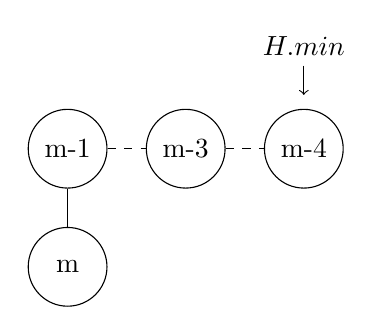
\begin{tikzpicture}[
      level 1/.style={sibling distance=48mm, level distance=10mm},
      level 2/.style={sibling distance=16mm, level distance=10mm},
      level 3/.style={sibling distance=8mm, level distance=10mm},
      node distance=1.5cm
    ]
    \node [circle,draw, minimum size=1cm] (1){m-1}
     child {node [circle,draw, minimum size=1cm, below of=1] (2){m}};
    \node [circle, draw, minimum size=1cm, right of=1] (4){m-3};
    \node [circle, draw, minimum size=1cm, right of=4] (5){m-4};
    \path [draw, dashed] (1)--(4);
    \path [draw, dashed] (4)--(5);
    \node [above of=5, yshift=-.2cm] (min) {$H.min$};
    \path [draw, ->, shorten >=5pt] (min)--(5.north);
    \end{tikzpicture}
    \end{figure}

    \textsc{Fib-Heap-Insert}(H, $m-5$):
    \begin{figure}[H]
    \centering
    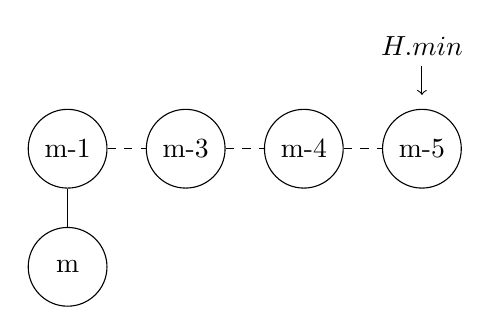
\begin{tikzpicture}[
      level 1/.style={sibling distance=48mm, level distance=10mm},
      level 2/.style={sibling distance=16mm, level distance=10mm},
      level 3/.style={sibling distance=8mm, level distance=10mm},
      node distance=1.5cm
    ]
    \node [circle,draw, minimum size=1cm] (1){m-1}
     child {node [circle,draw, minimum size=1cm, below of=1] (2){m}};
    \node [circle, draw, minimum size=1cm, right of=1] (4){m-3};
    \node [circle, draw, minimum size=1cm, right of=4] (5){m-4};
    \node [circle, draw, minimum size=1cm, right of=5] (6){m-5};
    \path [draw, dashed] (1)--(4);
    \path [draw, dashed] (4)--(5);
    \path [draw, dashed] (5)--(6);
    \node [above of=6, yshift=-.2cm] (min) {$H.min$};
    \path [draw, ->, shorten >=5pt] (min)--(6.north);
    \end{tikzpicture}
    \end{figure}

    \textsc{Fib-Heap-Extract-Min}(H):
    \begin{figure}[H]
    \centering
    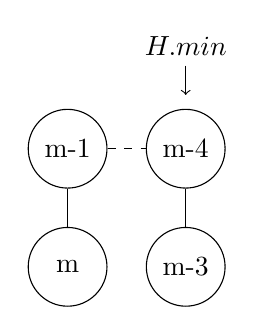
\begin{tikzpicture}[
      level 1/.style={sibling distance=48mm, level distance=10mm},
      level 2/.style={sibling distance=16mm, level distance=10mm},
      level 3/.style={sibling distance=8mm, level distance=10mm},
      node distance=1.5cm
    ]
    \node [circle,draw, minimum size=1cm] (1){m-1}
     child {node [circle,draw, minimum size=1cm, below of=1] (2){m}};
    \node [circle, draw, minimum size=1cm, right of=1] (4){m-4}
     child {node [circle, draw, minimum size=1cm, below of=4] (5){m-3}};
    \path [draw, dashed] (1)--(4);
    \path [draw, dashed] (4)--(5);
    \node [above of=4, yshift=-.2cm] (min) {$H.min$};
    \path [draw, ->, shorten >=5pt] (min)--(4.north);
    \end{tikzpicture}
    \end{figure}

    \textsc{Fib-Heap-Delete(H, $m-3$)}:
    \begin{figure}[H]
    \centering
    \begin{tikzpicture}[
      level 1/.style={sibling distance=48mm, level distance=10mm},
      level 2/.style={sibling distance=16mm, level distance=10mm},
      level 3/.style={sibling distance=8mm, level distance=10mm},
      node distance=1.5cm
    ]
    \node [circle, draw, minimum size=1cm, right of=1] (4){m-4}
     child {node [circle, draw, minimum size=1cm, below of=4] (5){m-1}
      child {node [circle,draw, minimum size=1cm, below of=5] (2){m}}};
    \node [above of=4, yshift=-.2cm] (min) {$H.min$};
    \path [draw, ->, shorten >=5pt] (min)--(4.north);
    \end{tikzpicture}
    \end{figure}

    \item \textbf{Solution:} \\
    \textbf{a.} The issue with the professor's claim is that while we can in
    fact add $x$'s child list to the root list of $H$ in constant time, this is
    not ``paying forward'' to the total amortized cost that it will take to do
    the eventual \textsc{Cascading-Cut}s that are necessary.

    \textbf{b.} The upper bound would be as bad as:

    $$ O(x.degree \cdot c) = O(\text{lg}n) $$

    \textbf{c.} The potential of $H$ might be:

    $$ \phi = x.degree \cdot c + \frac{t(H)}{m(H)} $$

    \textbf{d.} Thus, the amortized time for \textsc{Pisano-Delete} is no better
    than for \textsc{Fib-Heap-Delete}.

    \item \textbf{Solution:}
    We will use the stack, which we will call \texttt{stack}, to hold the actual
    element being inserted, and the ``huge'' array \texttt{dict} to hold
    references to where the element exists in \texttt{stack}. We will also need
    a ``mirrored'' stack, \texttt{mirrored}, which will hold the actual values
    of the elements. Since all actions are direct-access and of a constant
    number for each function, all functions are $O(1)$ running time.

    \textsc{Initialize}: At any given time, \texttt{stack} will contain
    exactly the number of elements that are currently stored in \texttt{dict}.
    Thus, at initialization, the size of \texttt{stack} is $0$, and requires no
    initialization. Since \texttt{dict} may contain garbage, and will only be
    overwritten, it too requires no initialization.

    \textsc{Insert}: When inserting a new element, we add the element to the
    end of \texttt{stack} as such:

    $$ \texttt{stack}[\texttt{stack}.length] = \texttt{element}.key $$

    We also add the value of the element to the mirrored stack:

    $$ \texttt{mirror}[\texttt{stack}.length] = \texttt{element}.value $$

    Since this increases the length of \texttt{stack} by $1$, the index of
    $\texttt{element}$ is now at $\texttt{stack}.length - 1$. We add this
    value to \texttt{dict}, overwriting whatever might be there.

    $$ \texttt{dict}[\texttt{element}.key] = \texttt{stack}.length - 1 $$

    \textsc{Search}: When searching for an \texttt{element}, we must satisfy two
    conditions to know that we will return the correct element in constant time.
    First, we must make sure that we have previously inserted this element and
    that the reference data in \texttt{dict} is not garbage:

    $$ 0 \leq \texttt{dict}[key] \leq \texttt{stack}.length -1 $$

    This alone, however, does not prove that \textsc{Search} is returning the
    correct element. We must also compare the results. The result is only valid
    if:

    $$ \texttt{stack}[\texttt{dict}[key]] = \texttt{key} $$

    If this is true, then we can return the value from the mirrored stack:

    $$ \texttt{mirrored}[\texttt{stack}[\texttt{dict}[key]]] $$

    \textsc{Delete}: Deletion can be done simply by turning the key reference in
    \texttt{dict} back into garbage, e.g. to a value that will never be a valid
    key and will fail the first test:

    $$ \texttt{dict}[key] = -1 $$

    This will leave a gap in \texttt{stack} (and in \texttt{mirror}). If it is
    desirable to maintain the lengths of these stacks to match the actual number
    of keys, we could maintain a separate stack which would keep track of
    deleted keys and re-use them when new elements are inserted.

    \item \textbf{Solution:}

    Assuming uniform hashing, given two elements $k$ and $l$ and a table of size
    $m$ the following probability is true for two elements, $k$ and $l$, where
    $k \neq l$ and $h(k) = h(l)$:

    $$ P_{individual-collision} = 1/m $$

    Thus the probability of not having a collision between $k$ and $l$ is:

    $$ P_{no-individual-collision} = 1 - P_{individual-collision} $$

    Therefore, the probability that there will be no collisions for a single
    element with any of the $n-1$ other elements is:

    $$ P_{never-collisions} = {P_{no-individual-collision}}^{(n-1)} $$

    Thus the probability that there will be at least one collision for a single
    element with any of the $n-1$ other elements is:

    $$ P_{collision} = 1 - P_{never-collisions} $$

    Therefore the expected number of collisions after inserting all $n$ nodes
    is:

    $$ n \cdot P_{collision} = n\left(1-\left(1-\frac{1}{m}\right)^{(n-1)}\right) $$

    \item \textbf{Solution:}
    For each set in $ \mathscr{H} $, the probability of there being a collision
    is $P_{collision}$ as was found in the previous question. The set $U$
    represents the number of available elements while the set $B$ represents the
    available locations without collisions. Thus the probability of there being
    a collision for any of the elements is:

    $$ P_{collision} \cdot \left( | B | - | U | \right) $$

    I'm not sure how to continue from there.
\end{enumerate}
\end{document}
